%%!TEX root = diss.tex

\chapter{Architecture}
\label{ch:Architecture}

% Add brief outline here.
This chapter outlines the proposed switch block memory architecture in comparison to baseline and prior work. Section \ref{arch:baseline} gives a brief background on how memory bits are used in contemporary switch block architecture. Section \ref{arch:limitations} details prior work's baseline switch block architecture and outlines why it cannot be directly ported over to contemporary switch block architectures. Section \ref{arch:proposed} outlines the proposed switch block memory architecture.

\section{Configuration bits within FPGA switch blocks}
\label{arch:baseline}
% \subsection{Current baseline FPGA switchblocks}
% This baseline talks about literally the baseline of modern fpga technology switchblock or the baseline of prior work?
% May need to move to background.
% Q: does it matter what switchblock you use? No. 
% Might be easier to think about with a disjoint switch block pattern since lemieux's paper uses disjoint
The baseline switch block architecture used in this thesis is from Versatile Place and Route (VPR) \cite{Murray2020VTRModelling}. 
For unidirectional segments, VPR uses a modified Wilton switch block pattern \cite{Wilton1997ArchitecturesMemory} in most cases. The Wilton switch block pattern is shown in Figure \ref{fig:wiltonswitchblock}, along with disjoint and universal patterns.
% Not sure if switch block patterns is necessary to talk about
\begin{figure}[!tb]
    \centering
    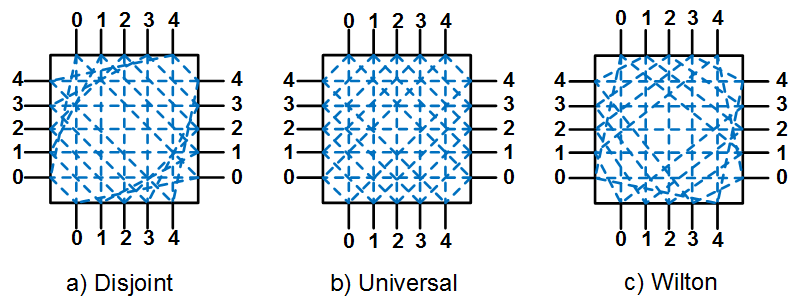
\includegraphics[width=0.33\textwidth]{fig/switchblocks.png}
    \caption{Wilton switch block pattern \cite{Yu2017FPGATargetability}}
    \label{fig:wiltonswitchblock}
\end{figure}

% Assume basics is talked about in background already
Regardless of the switch block pattern, a switch point within the switch block connects all four directions together, and is structured as in figure \ref{fig:switchblock}. Each switch point, depending on the switch architecture, can contain one or more switches.

% TODO: draw switch block.

A unidirectional switch architecture as seen in figure \ref{fig:uniswitch} is used as the baseline of our proposed work. We define a switch used inside a switch block as a switch point. In this case, the unidirectional switch point consists of four input and four output directions. For a given output direction, a 3:1 multiplexer is used to multiplex each of its three input directions together. Memory configuration bits are used to select the appropriate input direction for output. During configuration, these memory bits are written to only once.

% Bidirectional switch
% \begin{figure}[!htb]
% \centering
% \begin{circuitikz}[scale=0.4]
%     % mux
%     \draw (10,0) node[muxdemux, muxdemux def={Lh=4, Rh=1, NL=3, NB=0, NT=1, NR=1, w=2}, anchor=rpin 1](right_mux){};
%     \draw (-10,0) node[muxdemux, muxdemux def={Lh=1, Rh=4, NL=1, NB=0, NT=1, NR=3,w=2}, anchor=lpin 1](left_mux){};
%     \draw (0, -10) node[muxdemux, muxdemux def={Lh=1, Rh=4, NL=1, NB=0, NT=1, NR=3,w=2}, rotate=90, anchor=lpin 1](bot_mux){};
%     \draw (0, 10) node[muxdemux, muxdemux def={Lh=1, Rh=4, NL=1, NB=1, NT=0, NR=3,w=2}, rotate=-90, anchor=lpin 1](top_mux){};
%     % Buffers
%     \draw (right_mux.rpin 1) to[short] ++(1,0) node[ieeestd buffer port, anchor=in](right_buf){};
%     \draw (left_mux.lpin 1) to[short] ++(-1,0) node[ieeestd buffer port, xscale=-1, anchor=in](left_buf){};
%     \draw (bot_mux.lpin 1) to[short] ++(0,-1) node[ieeestd buffer port, anchor=in, rotate=-90](bot_buf){};
%     \draw (top_mux.lpin 1) to[short] ++(0,1) node[ieeestd buffer port, anchor=in, rotate=90](top_buf){};
%     \draw (right_buf.out) to[short,-o] ++(1,0);
%     \draw (top_buf.out) to[short,-o] ++(0,1);
%     \draw (left_buf.out) to[short,-o] ++(-1,0);
%     \draw (bot_buf.out) to[short,-o] ++(0,-1);
%     % Coordinates out of buf (WHEN MODIFYING SCALE THESE COORDINATES MAY NEED TO BE ADJUSTED)
%     \draw (right_buf.out) to[short] ++(0,-3.5) coordinate(right_out);
%     \draw (left_buf.out) to[short] ++(0,-3.5) coordinate(left_out);
%     \draw (top_buf.out) to[short] ++(3.5,0) coordinate(top_out);
%     \draw (bot_buf.out) to[short] ++(3.5,0) coordinate(bot_out);
%     % Horizontal lines + make dot coordinates
%     \draw (right_mux.lpin 1) to[short, -*] (right_mux.lpin 1 -| top_out) coordinate(dot1) to[short] (left_mux.rpin 1);
%     \draw (right_mux.lpin 2) to[short, -*]  (right_mux.lpin 2 -| top_mux.rpin 1) coordinate(dot2) to[short] (left_mux.rpin 2);
%     \draw (right_mux.lpin 3) to[short, -*] (right_mux.lpin 3 -| top_mux.rpin 2) coordinate(dot3);
%     % Vertical lines + make last dot coordinate
%     \draw (top_mux.rpin 3) to[short, -*] (top_mux.rpin 3 |- left_out) coordinate(dot4) to[short] (bot_mux.rpin 1);
%     \draw (top_mux.rpin 2) to[short] (bot_mux.rpin 2);
%     \draw (bot_mux.rpin 3) to[short] (dot2 |- dot1) to[short] ++(0,0.5) coordinate(t1);
%     \draw (top_mux.rpin 1) to[short] ++(0,-0.5) coordinate(t2);
%     % Buffer output coordinates to muxes
%     \draw (left_mux.rpin 3) to[short] ++(0.5,0) coordinate(r2);
%     \draw (right_out) to[short] (dot4) to[short] ++(-0.5,0) coordinate(r1) to[short] (r2);
%     \draw (left_out) to[short] (dot4 -| r2) to[short] (dot3 -| r1) to[short] (dot3);
%     \draw (bot_out) to[short] (dot1 |- t1) to[short] (t2);
%     \draw (top_out) to[short] (dot1 |- t2) to[short] (t1);
%     % SRAM boxes
%     \draw (top_mux.bpin 1) node [draw,align=center, anchor=e] {sram};
%     \draw (bot_mux.tpin 1) node [draw,align=center, anchor=e] {sram};
%     \draw (right_mux.tpin 1) node [draw,align=center, anchor=south] {sram};
%     \draw (left_mux.tpin 1) node [draw,align=center, anchor=south] {sram};    
% \end{circuitikz}
% \caption{Single bidirectional switch}
% \label{fig:biswitch}
% \end{figure}

% Unidirection switch
\begin{figure}[!htb]
\centering
\begin{circuitikz}[scale=0.4]
    % mux
    \draw (12,4) node[muxdemux, muxdemux def={Lh=4, Rh=1.5, NL=3, NB=0, NT=1, NR=1,w=1.5}, anchor=rpin 1](right_mux){};
    \draw (-12,-4) node[muxdemux, muxdemux def={Lh=1.5, Rh=4, NL=1, NB=0, NT=1, NR=3,w=1.5}, anchor=lpin 1](left_mux){};
    \draw (-4, -12) node[muxdemux, muxdemux def={Lh=1.5, Rh=4, NL=1, NB=0, NT=1, NR=3,w=1.5}, rotate=90, anchor=lpin 1](bot_mux){};
    \draw (4, 12) node[muxdemux, muxdemux def={Lh=1.5, Rh=4, NL=1, NB=1, NT=0, NR=3,w=1.5}, rotate=-90, anchor=lpin 1](top_mux){};
    % Buffers
    \draw (right_mux.rpin 1) to[short] ++(1,0) node[ieeestd buffer port, anchor=in,scale=0.75](right_buf){};
    \draw (left_mux.lpin 1) to[short] ++(-1,0) node[ieeestd buffer port, xscale=-1, anchor=in,scale=0.75](left_buf){};
    \draw (bot_mux.lpin 1) to[short] ++(0,-1) node[ieeestd buffer port, anchor=in, rotate=-90,scale=0.75](bot_buf){};
    \draw (top_mux.lpin 1) to[short] ++(0,1) node[ieeestd buffer port, anchor=in, rotate=90,scale=0.75](top_buf){};
    \draw (right_buf.out) to[short,-o] ++(1,0);
    \draw (top_buf.out) to[short,-o] ++(0,1);
    \draw (left_buf.out) to[short,-o] ++(-1,0);
    \draw (bot_buf.out) to[short,-o] ++(0,-1);
    % Drivers
    \draw (right_mux.lpin 1) 
    to[short, -*] (top_mux.rpin 3 |- right_mux.lpin 1) coordinate(r1)
    to[short, -*] (bot_mux.rpin 2 |- right_mux.lpin 1) coordinate(r0)
    to[short] (left_mux |- right_mux.lpin 1) coordinate (right_driver_out);
    \draw (right_driver_out) node[ieeestd buffer port, anchor=out,scale=0.5](right_driver){};
    \draw (right_driver.in) to[short,-o] ++(-1,0);   
    \draw (left_mux.rpin 3) 
    to[short, -*] (bot_mux.rpin 3 |- left_mux.rpin 3) coordinate(l1)
    to[short, -*] (top_mux.rpin 2 |- left_mux.rpin 3) coordinate(l0)
    to[short] (right_mux |- left_mux.rpin 3) coordinate (left_driver_out);
    \draw (left_driver_out) node[ieeestd buffer port, anchor=out,scale=0.5,xscale=-1](left_driver){};
    \draw (left_driver.in) to[short,-o] ++(1,0);
    \draw (bot_mux.rpin 1) 
    to[short, -*] (left_mux.rpin 1 -| bot_mux.rpin 1) coordinate(b1)
    to[short, -*] (right_mux.lpin 2 -| bot_mux.rpin 1) coordinate(b0)
    to[short] (top_mux -| bot_mux.rpin 1) coordinate (bot_driver_out);
    \draw (bot_driver_out) node[ieeestd buffer port, anchor=out,scale=0.5,rotate=-90](bot_driver){};
    \draw (bot_driver.in) to[short,-o] ++(0,1);
    \draw (top_mux.rpin 1) 
    to[short, -*] (right_mux.lpin 3 -| top_mux.rpin 1) coordinate(t1)
    to[short, -*] (left_mux.rpin 2 -| top_mux.rpin 1) coordinate(t0)
    to[short] (bot_mux -| top_mux.rpin 1) coordinate (top_driver_out);
    \draw (top_driver_out) node[ieeestd buffer port, anchor=out,scale=0.5,rotate=90](top_driver){};
    \draw (top_driver.in) to[short,-o] ++(0,-1);
    % Simple Connections
    \draw (top_mux.rpin 3) -- (r1);
    \draw (bot_mux.rpin 3) -- (l1);
    \draw (left_mux.rpin 1) -- (b1);
    \draw (right_mux.lpin 3) -- (t1);
    \draw (top_mux.rpin 2) -- (l0);
    \draw (bot_mux.rpin 2) -- (r0);
    \draw (left_mux.rpin 2) -- (t0);
    \draw (right_mux.lpin 2) -- (b0);
    % % SRAM boxes
    \draw (top_mux.bpin 1) node [draw,align=center, anchor=e] {sram};
    \draw (bot_mux.tpin 1) node [draw,align=center, anchor=e] {sram};
    \draw (right_mux.tpin 1) node [draw,align=center, anchor=south] {sram};
    \draw (left_mux.tpin 1) node [draw,align=center, anchor=south] {sram};      

\end{circuitikz}
\caption{Single unidirectional switch}
\label{fig:uniswitch}
\end{figure}

\subsection{Baseline multiplexer architecture}
\label{arch:mux_arch}
The number of configuration bits used within the unidirectional switch point's multiplexer can differ depending on its  circuitry.
There are two cases.
The first case is simple; the number of configuration bits used ties directly to the number of multiplexer inputs. For 3 multiplexer inputs, there are 3 configuration bits, as shown in figure \ref{fig:simple_mux}.
% TODO: change up the multiplexer SRAM bits because they are not just a single transistor in this diagram?
% Basic mux arch where 3 bits control 3 lines
\begin{figure}[!htb]
    \centering
    \begin{circuitikz}
        \draw (0,0) node[muxdemux, muxdemux def={Lh=4, Rh=1, NL=3, NB=0, NT=1, NR=1}](mux){};
        \draw (-2, 3) node[nmos](t1){};
        \draw (0, 3) node[nmos](t2){};
        \draw (2, 3) node[nmos](t3){};
        \draw (t1.S) to[short] ++(0,-0.25) to[short] ++(4,0);
        \draw (t2.S) to[short] ++(0,-0.25) to[short] ++(0,0);
        \draw (t3.S) to[short] ++(0,-0.25) to[short] ++(0,0);
        \draw (mux.tpin 1) to[short] ++(0,1);
        \draw (t1.D) to[short, -o] ++(0,.25);
        \draw (t2.D) to[short, -o] ++(0,.25);
        \draw (t3.D) to[short, -o] ++(0,.25);
    \end{circuitikz}
    \caption{Simple multiplexer using 3 configuration memory bits}
    \label{fig:simple_mux}
\end{figure}

The second case reduces the number of configuration bits by using an intermediate decoder. The decoder in figure \ref{fig:decoder_new} allows compressing the number of input directions by $log_2$. 2 configuration bits can be used to control 4 input lines, shown in figure \ref{fig:decoder_mux}. We consider this structure as the baseline as it minimizes the number of configuration memory bits.
% the existing circuitry used to read/write to the two configuration memory bits of a bidirectional track can be used to read/write to the two configuration memory bits of an unidirectional track. Further, since the unidirectional track splits up the bidirectional track in two. This is shown in figure \ref{fig:proposed_arch}. 

% Decoder_mux
\begin{figure}[!htb]
    \centering
    \begin{circuitikz}
        \draw (0,0) node[muxdemux, muxdemux def={Lh=4, Rh=1, NL=3, NB=0, NT=1, NR=1}](mux){};
        \draw (-1, 5) node[nmos](t1){};
        \draw (1, 5) node[nmos](t3){};
        \draw (t1.S) to[short] ++(0,-0.25) to[short] ++(2,0);
        \draw (t3.S) to[short] ++(0,-0.25) to[short] ++(0,0);
        \draw (mux.tpin 1) to[short] ++(0,1) node [draw,align=center, anchor=south](dec) {decoder};
        \draw (dec.north) to[short] ++(0,1.47);
        \draw (t1.D) to[short, -o] ++(0,.25);
        \draw (t3.D) to[short, -o] ++(0,.25);
    \end{circuitikz}
    \caption{2 bits of configuration memory using a decoder + 3:1 multiplexer}
    \label{fig:decoder_mux}
\end{figure}

4 decoder outputs are possible with two bits of configuration memory, although in the baseline unidirectional switch configuration only 3 are used since there are 3 inputs into the multiplexer. We assume there exists a 4th input as ground, since it is unlikely that during normal switch point operation all outputs are driven regardless of use.

\begin{figure}[!htb]
    \centering
    \begin{circuitikz}
        \draw (1,0.5) node [draw, align=center, anchor=south](sram){sram[1:0]};
        \draw (0,0) to[short, o-] ++(0,-1) node[ieeestd not port, rotate=-90, anchor=in](not1){};       
        \draw (2,0) to[short, o-] ++(0,-1) node[ieeestd not port, rotate=-90, anchor=in](not2){};
        % First and gate
        \draw (not2.out) to[short, -*] ++(0,-1) to[short] ++(1,0) node[ieeestd and port, anchor=in 1](and1){}; 
        \draw (not1.out) to[short, -*] ++(0,-1.56) to[short] (and1.in 2);
        % Second and gate
        \draw (not2.in) to[short] ++(-1,0) to[short,-*] ++(0,-4.5)  coordinate(and4_start1) to[short] ++(2,0)  node[ieeestd and port, anchor=in 1](and2){};
        \draw (not1.out) to[short] ++(0,-3.3) to[short] (and2.in 2);
        % Third and gate
        \draw (not1.in) to[short] ++(-1,0) to[short,-*] ++(0,-6.25)  coordinate(and4_start2) to[short] ++(4,0)  node[ieeestd and port, anchor=in 1](and3){};
        \draw (not2.out) to[short] ++(0,-5.06) to[short] (and3.in 2);
        % Fourth and gate
        \draw (and4_start1) to[short] ++(0,-3.5) to[short] ++(2,0) node[ieeestd and port, anchor=in 1](and4){};
        \draw (and4_start2) to[short] (and4_start2 |- and4.in 2) to[short] (and4.in 2);
    \end{circuitikz}
        \caption{2:4 decoder structure}
    \label{fig:decoder_new}
\end{figure}

% Note that in regards to area, the number of transistors for the multiplexer decoder is the same for the unmodified baseline versus with the proposed circuitry, since the decoder circuitry is not modified.

\section{The bidirectional track architecture}
\label{arch:limitations}
% Limitations of baseline, including that it was done on older technology and bidirectional wires.
% Section \ref{bg:wideshallowmem} provides an introductory background into prior work. 
This section details the bidirectional track architecture and how it is used in prior work for comparison with the proposed architecture in the following section \ref{arch:proposed}. 

A bidirectional switch point considered in prior work as seen in figure \ref{fig:bidirectional_switchpoint}, has 1 horizontal connection, 1 vertical connection, and 4 diagonal connections for a total of 6 connections possible. All of these connections are implemented within a switch point. Each switch connection (figure \ref{fig:prior_baseline} consists of a bidirectional driver made up of 2 tri-state buffers. Each tri-state is controlled by one configuration bit memory. In prior work, the horizontal and vertical connections are used and left unmodified to allow for memory input and output of the switch point to connect to the switch block external pins. The 4 diagonal connections are modified to access the 2 configuration bits. In the original baseline, the 4 diagonal connections' configuration bits would be unused when the horizontal and vertical connections are used.

Prior work's bidirectional switch architecture, depicted in figure \ref{fig:prior_arch}, modifies the baseline bidirectional switch (figure \ref{fig:prior_baseline} to take advantage of the unused configuration memory within these diagonal connections. By adding pass transistors to the switch, the configuration memory can be both read out and written to. More specifically, disconnecting the diagonal connections is made possible by adding, then turning off, a pass transistor in the critical path of the bidirectional connection as seen in figure \ref{fig:prior_arch}.

Figure \ref{fig:prior_control} shows prior work's memory addressing and control circuitry. As mentioned, the vertical and horizontal switches cannot be used as memory since the tracks they implement are used to connect to the address decoder or to access the configuration memory. This means that only the diagonal connections are able to be read and written to. Further, this makes up 8 bits of accessible memory per switch point and corresponds to a memory depth of 8.  The lower right of figure \ref{fig:prior_control} shows the disconnected 4 diagonal connections possible that allow for memory to be read out or written to. Since only the diagonal switches within a switch block are modified to allow for access in all directions, all non-diagonal switches are kept in its vertical and horizontal connection configuration, allowing for this connection. Lastly, the tri-state drivers in the horizontal and vertical track directly turn off unused inputs and outputs, reducing power.

% Prior arch
\begin{figure}[!htb]
\begin{center}
\begin{circuitikz}[scale=1]
    % Pass transistor + sram write transistor
    \draw (0, 0) node[nmos, rotate=-90](p1){} ++(0,1) to[short] ++(0,1) node[nmos, anchor=S](t1){};
    % sram sel transistor
    \node [nmos,rotate=-90,anchor=D](t2) at (t1.D){};
    % sram Inverters
    \node [ieeestd not port, anchor=in](a1) at (t1.D){};
    \node [ieeestd not port, rotate=-180, anchor=out](a2) at (t1.S){};
    % Connect sram inverters
    \draw (a2.in) to (a1.out);
    % sram Labels
    \draw (t1.G) to[short,l=write] ++(0,0);
    \draw (t2.G) to[short,l=select] ++(0,0);
    \draw (t2.S) to[short,l=to config lines] ++(0,0);
    % Tri state
    \node[blue] [nmos, rotate=-90, anchor=D](p3) at (p1.S){};
    \node [ieeestd not port, anchor=out](a3) at (p3.S){};
    \node [ieeestd not port, anchor=out](a4) at (a3.in){};
    \draw (a4.in) to[short] ++(0,-2);
    \draw (p1.D) to[short] ++(0,-2) node[ieeestd not port, xscale=-1,anchor=in](a5){};
    \node [ieeestd not port, xscale=-1, anchor=in](a6) at (a5.out){};
    \node[blue] [nmos, rotate=90, anchor=S](p4) at (a6.out){};
    \node [nmos, rotate=90, anchor=S](p2) at (p4.D){};
    % Draw 2nd sram below
    \draw (p2.G) to[short] ++(0,-1) node[nmos, xscale=-1, anchor=D](t3){};
    % sram sel transistor
    \node [nmos,rotate=-90,xscale=-1,anchor=S](t4) at (t3.S){};
    % sram Inverters
    \node [ieeestd not port,anchor=out](a3) at (t3.D){};
    \node [ieeestd not port,xscale=-1,anchor=in](a4) at (t3.S){};
    % Connect sram inverters
    \draw (a3.in) to (a4.out);
    % sram Labels
    \draw (t3.G) to[short,l=write] ++(0.3,0);
    \draw (t4.G) to[short,l=select] ++(0,0);
    \draw (t4.D) to[short,l=to config lines] ++(1,0);
    % transistor labels
    \draw[blue] (p3.G) to[short, l=!M] ++(0,0);
    \draw[blue] (p4.G) to[short, l=!M] ++(0,0);
    % to other tracks
    \draw[blue] (t1.D) to[short] ++(0,1) to[short] ++(2,0) node[nmos, rotate=-90,anchor=S](w1){};
    \draw[blue] (w1.D) to[short] ++(0.5,0) to[short] ++(0,-3) node[nmos, rotate=-90, anchor=S](w2){};
    \draw[blue] (w2.G) ++(2,0) to[short,l=MemVert] ++(0,0);
    \draw[blue] (w2.D) ++(2.5,0) to[short, l=vertical track] ++(0,0);
    \draw[blue] (w2.S) to[short] ++(0,-3) node[nmos, rotate=-90, anchor=S](w3){};
    \draw[blue] (w3.D) ++(3,0) to[short, l=horizontal track] ++(0,0);
    \draw[blue] (w3.G) ++(2,0) to[short,l=MemHorz] ++(0,0);
    \draw[blue] (t4.S) to[short] ++(0,-2) to[short] ++(7,0) node[nmos, rotate=-90,anchor=S](w4){};
    \draw[blue] (w4.D) to[short] ++(0.525,0) to[short] (w3.S);
    \draw[blue] (w1.G) to[short, l=AS1] ++(0,0);
    \draw[blue] (w4.G) to[short, l=AS2] ++(0,0);
    \end{circuitikz}
\caption{Prior work's bidirectional connection, enhanced programmable connection in blue}
\label{fig:prior_arch}
\end{center}
\end{figure}

% Prior work's control/address circuitry figure
\begin{figure}[!htb]
\begin{center}
\begin{circuitikz}[scale=1]
    % Decoder
    \draw (0,0) node[muxdemux, muxdemux def={Lh=8, Rh=8, w=4, NL=8, NB=3, NT=0, NR=0}, anchor=lpin 1](decoder){3:8 decoder};
    % Decoder labels
    \draw (decoder.lpin 3) to[short, l=AS1(3..0)] ++(0,0);
    \draw (decoder.lpin 6) to[short, l=AS2(3..0)] ++(0,0);
    % Address labels
    \draw (decoder.bpin 1) ++(0,-0.5) to[short, l=A0] ++(0,0);
    \draw (decoder.bpin 2) ++(0,-0.5) to[short, l=A1] ++(0,0);
    \draw (decoder.bpin 3) ++(0,-0.5) to[short, l=A2] ++(0,0);
    % Address pins
    \draw (decoder.bpin 1) to[short] ++(0,-4) coordinate(h1);
    \draw (decoder.bpin 2) to[short] ++(0,-4) coordinate(h2);
    \draw (decoder.bpin 3) to[short] ++(0.25,0) to[short] ++(0,-1) coordinate(a2in);
    % A2 and lines
    \draw (a2in) node[muxdemux, muxdemux def={Lh=2, Rh=1, w=1, NL=2, NB=1, NT=0, NR=1}, anchor=rpin 1, rotate=90](a2mux){};
    \draw (a2mux.bpin 1) ++(1,0) to[short,l=bit 2] ++(0,0);
    % Vertical track
    \draw (a2mux.lpin 2) 
    to[short]       ++(2  ,0) coordinate(v0)
    to[short, -*]   ++(0.5,0) coordinate(v1) 
    to[short]       ++(0.5,0) coordinate(v2) 
    to[short]       ++(0.5,0) coordinate(v3) 
    to[short]       ++(0.5,0) coordinate(v4)
    to[short, -*]   ++(0.5,0) coordinate(v5)
    to[short]       ++(0.5,0) coordinate(v6)
    to[short]       ++(0.5,0) coordinate(v7)
    to[short]       ++(0.5,0) coordinate(v8)
    to[short]       ++(0.25,0) coordinate(v9);
    \draw (v0) 
    to[short, -*]   ++(0, -0.5) coordinate(vl0)
    to[short]       ++(0, -0.25) coordinate(arrow1)
    to[short]       ++(0, 0.75) coordinate(vl1)
    to[short]       ++(0, 0.5)  coordinate(vl2)
    to[short]       ++(0, 0.5)  coordinate(vl3)
    to[short]       ++(0,3);
    \draw (v1) 
    to[short]       ++(0, -0.5)
    to[short]       ++(0, -0.25) 
    to[short]       ++(0, 0.75)
    to[short]       ++(0, 0.5)
    to[short]       ++(0, 0.5)
    to[short]       ++(0,3);
    \draw (v2) 
    to[short]       ++(0, -0.5)
    to[short]       ++(0, -0.25) coordinate(line0)
    to[short]       ++(0, 0.75)
    to[short, -*]   ++(0, 0.5)
    to[short]       ++(0, 0.5)
    to[short]       ++(0,3);
    \draw (v3) 
    to[short]       ++(0, -0.5)
    to[short]       ++(0, -0.25) 
    to[short]       ++(0, 0.75)
    to[short]       ++(0, 0.5)
    to[short, -*]   ++(0, 0.5)
    to[short]       ++(0,3);
    \draw (v4) 
    to[short, -*]   ++(0, -0.5)
    to[short]       ++(0, -0.25) coordinate(line1)
    to[short]       ++(0, 0.75)
    to[short]       ++(0, 0.5)
    to[short]       ++(0, 0.5)
    to[short]       ++(0,3);
    \draw (v5) 
    to[short]       ++(0, -0.5)
    to[short]       ++(0, -0.25) coordinate(arrow2)
    to[short]       ++(0, 0.75)
    to[short]       ++(0, 0.5)
    to[short]       ++(0, 0.5)
    to[short]       ++(0,3);
    \draw (v6) 
    to[short]       ++(0, -0.5)
    to[short]       ++(0, -0.25) 
    to[short]       ++(0, 0.75)
    to[short,-*]    ++(0, 0.5)
    to[short]       ++(0, 0.5)
    to[short]       ++(0,3);
    \draw (v7) 
    to[short]       ++(0, -0.5)
    to[short]       ++(0, -0.25) 
    to[short]       ++(0, 0.75)
    to[short]       ++(0, 0.5)
    to[short,-*]    ++(0, 0.5)
    to[short]       ++(0,3);
    \draw (v8) 
    to[short]       ++(0, -0.5) coordinate(ve0)
    to[short]       ++(0, -0.25)
    to[short]       ++(0, 0.75) coordinate(ve2)
    to[short]       ++(0, 0.5)  coordinate(ve3)
    to[short]       ++(0, 0.5)  coordinate(ve4)
    to[short]       ++(0,3) ++(0,0.5) to[short, l=Vertical routing tracks] ++(0,0);
    \draw (vl0) to[short] (ve0) to[short] ++(0.25,0);
    \draw (vl1) to[short] (ve2) to[short] ++(0.25,0);
    \draw (vl2) to[short] (ve3) to[short] ++(0.25,0);
    \draw (vl3) to[short] (ve4) to[short] ++(0.25,0);
    % Horizontal track
    \draw (a2mux.lpin 1) to[short] (h2 -| a2mux.lpin 1) coordinate(h3);
    \draw (h2) to[short] ++(2.5,0) coordinate(arrow1end) to[short] ++(4,0) coordinate(hend); 
    \draw (h2) to[short, -*] ++(-1.5,0) coordinate(h0) to[short] ++(-3,0) coordinate(hstart);
    \draw (h0) to[short] ++(0,-0.5) coordinate(l1)
    to[short] ++(0,-0.5) coordinate(l2)
    to[short] ++(0,-0.5) coordinate(l3)
    to[short, -*] ++(0,-0.5) coordinate(l4)
    to[short] ++(0,-0.5) coordinate(l5)
    to[short] ++(0,-0.5) coordinate(l6)
    to[short] ++(0,-0.5) coordinate(l7)
    to[short] ++(0,-0.5) coordinate(l8)
    to[short] ++(0,-0.5) coordinate(l9);
    \draw (h1) to[short] (l9 -| h1);
    \draw (h2) to[short] (l9 -| h2);
    \draw (h3) to[short] (l9 -| h3);
    \draw (l1) to[short, -*] (l1 -| h1) to[short] ++(2,0) coordinate(hend1);
    \draw (l1) to[short] (l1 -| hstart);
    \draw (l2) to[short, -*] (l2 -| h2) to[short] (l2 -| hend1);
    \draw (l2) to[short] (l2 -| hstart);
    \draw (l3) to[short, -*] (l3 -| h3) to[short] (l3 -| hend1);
    \draw (l3) to[short] (l3 -| hstart);
    \draw (l4) to[short, -*] (l4 -| h0) to[short] (l4 -| hend1);
    \draw (l4) to[short] (l4 -| hstart);
    \draw (l5) to[short, -*] (l5 -| h1) to[short] (l5 -| hend1);
    \draw (l5) to[short] (l5 -| hstart);
    \draw (l6) to[short, -*] (l6 -| h2) to[short] (l6 -| hend1);
    \draw (l6) to[short] (l6 -| hstart);
    \draw (l7) to[short, -*] (l7 -| h3) to[short] (l7 -| hend1);
    \draw (l7) to[short] (l7 -| hstart);
    \draw (l8) to[short, -*] (l8 -| h0) to[short] (l8 -| hend1);
    \draw (l8) to[short] (l8 -| hstart)
    ++(3, -0.5)to[short, l=Horizontal routing tracks] ++(0,0);
    % Circuitry
    \draw (h0) to[short] ++(0,2) to[short] ++(-2,0) node[ieeestd xor port, anchor=in 1, xscale=-1,scale=0.5](xor){};
    \draw (xor.in 2) ++(1,-0.05) to[short, l=bit 2] ++(0,0);
    \draw (xor.out) to[short] ++(-0.25,0) to[short] ++(0,0.25) node[ieeestd and port, anchor=in 2, rotate=90, scale=0.5](and){};
    \draw(and.out) to[short] ++(0,1.1) ++(0,0) to[short, l=MemVert] ++(0,0);
    \draw (and.out) to[short] ++(0.5,0) node[ieeestd not port, anchor=in, rotate=90,scale=0.5](not0){};
    \draw (not0.out) to[short] ++(0,0.25) ++(2,0) to[short,l=MemHorz] ++(0,0);
    \draw (and.in 1) to[short] ++(0,-1.5) to[short,l=bit 1] ++(0,0);
    \draw (and.in 1) to[short] ++(0,-0.5) to[short] ++(-1,0) to[short] ++(0,0.25) node[ieeestd not port, anchor=in, rotate=90, scale=0.5](not1){};
    \draw (not1.out) to[short,l=!M] ++(0,0);
    % Arrows
    \draw [latexslim-latexslim,scale=2] (arrow1) -- (arrow1end);
    \draw [latexslim-latexslim,scale=2] (arrow2) -- (hend);
    \draw (line0) ++(0,-2) coordinate(arrow3);
    \draw (arrow3) to[short] ++(0,-1);
    \draw (line1) ++(0,-2) coordinate(arrow4);
    \draw (arrow4) to[short] ++(0,-1);
    \draw [latexslim-latexslim,scale=2] (arrow3) -- (hend);
    \draw [latexslim-latexslim,scale=2] (arrow4) -- (arrow1end);

    \end{circuitikz}
\caption{Prior work's addressing and control circuitry, only the A2 multiplexer is shown for simplicity}
\label{fig:prior_control}
\end{center}
\end{figure}

For each switch block the memory is made addressable by delegating 3 track lines as address lines. This controls the AS1 and AS2 pass transistors. Following these address transistors is an intermediate staging area, connected to the horizontal and vertical track via two more pass transistors controlled using 1 control line. In total, 4 track lines comprises A0-A2 (for a memory depth of 8 since $log_2(8)=3$) and a control line to select MemVert, MemHorz, and M. MemVert and MemHorz control the input/output track direction while M selects usage of the switch block as a memory or regular switch block and is controlled by bit 1. Bit 1 and 2 come from two configuration bits, a necessary overhead per switch block. Bit 2 controls the logic that selects between a horizontal track input or vertical track input. Accordingly, if used as memory, the output is selected to be the other track. 
This allows for memory access to the now user-accessible memories within these diagonal switches. 
% Since these drivers no longer form a loop within the same switch, much more flexibility can be added into the memory addressing and control. This can be seen by comparing address and control circuitry.

However, the configuration memory made accessible in prior work specifically targets a bidirectional architecture using tri-state inverters. In more modern architectures, the tri-state buffers are removed in favour for multiplexers in a unidirectional manner. Since prior work modifies the architecture of the tri-state buffers within the switch block to be able to be read out and written to, this can no longer be feasible. 

\section{The unidirectional switch (and why directly mapping prior work doesn't work)}
% TODO: include in overhead calculation
In a unidirectional switch, instead of reading and writing to the tri-state buffer's configuration memory, the multiplexer's configuration memory is used instead. Seen in figure \ref{fig:uniswitch}, this configuration memory is used to multiplex one of three incoming input directions to its output direction. The fourth input direction (not-depicted) is connected to ground when not in use.

\begin{figure}
    \begin{circuitikz}
% left tracks
    \draw(1,0) to[short,-o] (5,0) coordinate(l0);
    \draw(1,1) to[short,-o] (4,1) coordinate(l1);
    \draw(1,2) to[short,-o] (3,2) coordinate(l2);
    \draw(1,3) to[short,-o] (2,3) coordinate(l3);
% right tracks
    \draw(7,0) to[short,-o] (6,0) coordinate(r0);
    \draw(7,1) to[short,-o] (5,1) coordinate(r1);
    \draw(7,2) to[short,-o] (4,2) coordinate(r2);
    \draw(7,3) to[short,-o] (3,3) coordinate(r3);
% bot tracks
    \draw(5.5,-1) to[short,-o] (5.5,-0.5) coordinate(b0);
    \draw(4.5,-1) to[short,-o] (4.5,0.5) coordinate(b1);
    \draw(3.5,-1) to[short,-o] (3.5,1.5) coordinate(b2);
    \draw(2.5,-1) to[short,-o] (2.5,2.5) coordinate(b3);
% top tracks
    \draw(5.5,4) to[short,-o] (5.5,0.5)coordinate(t0);
    \draw(4.5,4) to[short,-o] (4.5,1.5)coordinate(t1);
    \draw(3.5,4) to[short,-o] (3.5,2.5)coordinate(t2);
    \draw(2.5,4) to[short,-o] (2.5,3.5)coordinate(t3);

% Direct connections
\draw[blue] (l0) to[short] (r0);
\draw[blue] (l1) to[short] (r1);
\draw[blue] (l2) to[short] (r2);
\draw[blue] (l3) to[short] (r3);
\draw[blue] (t0) to[short] (b0);
\draw[blue] (t1) to[short] (b1);
\draw[blue] (t2) to[short] (b2);
\draw[blue] (t3) to[short] (b3);
% Diagonal connections
\draw[blue, densely dotted] (l0) to[short] (t0);
\draw[blue, densely dotted] (l1) to[short] (t1);
\draw[blue, densely dotted] (l2) to[short] (t2);
\draw[blue, densely dotted] (l3) to[short] (t3);
\draw[blue, densely dotted] (t0) to[short] (r0);
\draw[blue, densely dotted] (t1) to[short] (r1);
\draw[blue, densely dotted] (t2) to[short] (r2);
\draw[blue, densely dotted] (t3) to[short] (r3);
\draw[blue, densely dotted] (r3) to[short] (b3);
\draw[blue, densely dotted] (r2) to[short] (b2);
\draw[blue, densely dotted] (r1) to[short] (b1);
\draw[blue, densely dotted] (r0) to[short] (b0);
\draw[blue, densely dotted] (b0) to[short] (l0);
\draw[blue, densely dotted] (b1) to[short] (l1);
\draw[blue, densely dotted] (b2) to[short] (l2);
\draw[blue, densely dotted] (b3) to[short] (l3);

% Switch block outline
\draw[red, thick] (1.5,-0.75) to[short] (6.5,-0.75) to[short] (6.5,3.75) to[short] (1.5,3.75) to[short] (1.5,-0.75);
    \end{circuitikz}
\caption{Bidirectional switch points (blue) within a switch block (red), where each switch point is capable of 6 switch connections}
\label{fig:bidirectional_switchpoint}
\end{figure}

\begin{figure}
 \begin{circuitikz}
% left tracks
    \draw(1,0) to[short,-*] (5,0) coordinate(l00);
    \draw(1,0.5) to[short,-o] (5,0.5) coordinate(l0);
    \draw(1,1) to[short,-*] (4,1) coordinate(l11);
    \draw(1,1.5) to[short,-o] (4,1.5) coordinate(l1);
    \draw(1,2) to[short,-*] (3,2) coordinate(l22);
    \draw(1,2.5) to[short,-o] (3,2.5) coordinate(l2);
    \draw(1,3) to[short,-*] (2,3) coordinate(l33);
    \draw(1,3.5) to[short,-o] (2,3.5) coordinate(l3);
% right tracks
    \draw(7,0) to[short,-o] (6,0) coordinate(r0);
    \draw(7,0.5) to[short,-*] (6,0.5) coordinate(r00);
    \draw(7,1) to[short,-o] (5,1) coordinate(r1);
    \draw(7,1.5) to[short,-*] (5,1.5) coordinate(r11);
    \draw(7,2) to[short,-o] (4,2) coordinate(r2);
    \draw(7,2.5) to[short,-*] (4,2.5) coordinate(r22);
    \draw(7,3) to[short,-o] (3,3) coordinate(r3);
    \draw(7,3.5) to[short,-*] (3,3.5) coordinate(r33);
% bot tracks
    \draw(5.25,-0.75) to[short,-o] (5.25,-0.25) coordinate(b0);
    \draw(4.25,-0.75) to[short,-o] (4.25,0.75) coordinate(b1);
    \draw(3.25,-0.75) to[short,-o] (3.25,1.75) coordinate(b2);
    \draw(2.25,-0.75) to[short,-o] (2.25,2.75) coordinate(b3);
    \draw(5.75,-0.75) to[short,-*] (5.75,-0.25) coordinate(b00);
    \draw(4.75,-0.75) to[short,-*] (4.75,0.75) coordinate(b11);
    \draw(3.75,-0.75) to[short,-*] (3.75,1.75) coordinate(b22);
    \draw(2.75,-0.75) to[short,-*] (2.75,2.75) coordinate(b33);
% top tracks
    \draw(5.75,4.25) to[short,-o] (5.75,0.75)coordinate(t0);
    \draw(4.75,4.25) to[short,-o] (4.75,1.75)coordinate(t1);
    \draw(3.75,4.25) to[short,-o] (3.75,2.75)coordinate(t2);
    \draw(2.75,4.25) to[short,-o] (2.75,3.75)coordinate(t3);
    \draw(5.25,4.25) to[short,-*] (5.25,0.75)coordinate(t00);
    \draw(4.25,4.25) to[short,-*] (4.25,1.75)coordinate(t11);
    \draw(3.25,4.25) to[short,-*] (3.25,2.75)coordinate(t22);
    \draw(2.25,4.25) to[short,-*] (2.25,3.75)coordinate(t33);

% Direct connections
\draw[blue] (l0) to[short] (r00);
\draw[blue] (l1) to[short] (r11);
\draw[blue] (l2) to[short] (r22);
\draw[blue] (l3) to[short] (r33);
\draw[blue] (t0) to[short] (b00);
\draw[blue] (t1) to[short] (b11);
\draw[blue] (t2) to[short] (b22);
\draw[blue] (t3) to[short] (b33);
\draw[blue] (l00) to[short] (r0);
\draw[blue] (l11) to[short] (r1);
\draw[blue] (l22) to[short] (r2);
\draw[blue] (l33) to[short] (r3);
\draw[blue] (t00) to[short] (b0);
\draw[blue] (t11) to[short] (b1);
\draw[blue] (t22) to[short] (b2);
\draw[blue] (t33) to[short] (b3);
% Diagonal connections
\draw[blue, densely dotted] (l0) to[short] (t00);
\draw[blue, densely dotted] (l1) to[short] (t11);
\draw[blue, densely dotted] (l2) to[short] (t22);
\draw[blue, densely dotted] (l3) to[short] (t33);
\draw[blue, densely dotted] (t0) to[short] (r00);
\draw[blue, densely dotted] (t1) to[short] (r11);
\draw[blue, densely dotted] (t2) to[short] (r22);
\draw[blue, densely dotted] (t3) to[short] (r33);
\draw[blue, densely dotted] (r3) to[short] (b33);
\draw[blue, densely dotted] (r2) to[short] (b22);
\draw[blue, densely dotted] (r1) to[short] (b11);
\draw[blue, densely dotted] (r0) to[short] (b00);
\draw[blue, densely dotted] (b0) to[short] (l00);
\draw[blue, densely dotted] (b1) to[short] (l11);
\draw[blue, densely dotted] (b2) to[short] (l22);
\draw[blue, densely dotted] (b3) to[short] (l33);
\draw[blue, densely dotted] (l00) to[short] (t0);
\draw[blue, densely dotted] (l11) to[short] (t1);
\draw[blue, densely dotted] (l22) to[short] (t2);
\draw[blue, densely dotted] (l33) to[short] (t3);
\draw[blue, densely dotted] (t00) to[short] (r0);
\draw[blue, densely dotted] (t11) to[short] (r1);
\draw[blue, densely dotted] (t22) to[short] (r2);
\draw[blue, densely dotted] (t33) to[short] (r3);
\draw[blue, densely dotted] (r33) to[short] (b3);
\draw[blue, densely dotted] (r22) to[short] (b2);
\draw[blue, densely dotted] (r11) to[short] (b1);
\draw[blue, densely dotted] (r00) to[short] (b0);
\draw[blue, densely dotted] (b00) to[short] (l0);
\draw[blue, densely dotted] (b11) to[short] (l1);
\draw[blue, densely dotted] (b22) to[short] (l2);
\draw[blue, densely dotted] (b33) to[short] (l3);

% Switch block outline
\draw[red, thick] (1.5,-0.5) to[short] (6.5,-0.5) to[short] (6.5,4) to[short] (1.5,4) to[short] (1.5,-0.5);
    \end{circuitikz}
\caption{Unidirectional switch points (blue) within a switch block (red), where each switch is capable of 8 switch connections}
\label{fig:unidirectional_switchpoint}
\end{figure}

A unidirectional switch point, seen in figure \ref{fig:uniswitch} and figure \ref{fig:unidirectional_switchpoint}, has the possibility of 2 horizontal connections, 2 vertical connections, and 8 diagonal connections for a total of 12 possible switch connections. In contrast to the bidirectional switch point, not all connections are used, since the multiplexer selection results in only 8 connections connected at a time. As a result of the multiplexer simplifying and consolidating the total number of connections used, disconnecting only the 4 diagonal connections as done in prior work to allow for configuration memory access is no longer possible. Keeping the horizontal and vertical tracks in a normal usage configuration would mean that all 4 multiplexers are configured, leaving no possibility for any configuration memory to be open for access. This is effectively an unmodified unidirectional switch point. 

% and to minimize changes to this control circuit we can mimic the same structure of the bidirectional switch and assume that all horizontal (and all vertical) tracks are connected and staggered in the same way as in prior work. 

That being said, the unidirectional switch opens up a larger possibility of configuration memory switch structures. In prior work's bidirectional switch point, the diagonal switch connections are used as configuration memory.
This limits the possible input/output track choices to two. If the horizontal switch track is chosen to be the input, the other vertical switch track must be an output, and vice-versa.
On the other hand, the unidirectional switch allows for a finer selection granularity between the input and output track choices, since the input and output tracks are decoupled. This results in a possible total number of input/output track permutations of 16, because for every one (of four) input directions there are 4 output direction tracks possible. 
% Future work: although preserving the same diagonal structure is possible, there is no limitation to using diagonal switch points 

Therefore, having an input and output coming and leaving in any of the four directions is possible. An input and output coming from the same direction should be made possible, although unlikely in practice due to issues such as congestion. In order to keep such flexibility the proposed architecture must also be highly flexible. This also makes multi-ported memory possible, with multiple inputs or outputs. For sake of simplicity however we will consider only single-ported memory since additional circuitry to control multi-ported behaviour is much more complicated and adds extra overhead.

This flexibility increases the number of permutations further by varying the amount of user accessible configuration bits per switch point. Each multiplexer within the switch point has two bits of configuration memory, which can be either configured as user-accessible, leaving the multiplexer unused, or configured as normal operation, allowing for normal routing purposes. The use of such a hybrid configuration could potentially alleviate routing problems in the CAD flow. 

Exploring such an exhaustive list of the possible input/output memory switch connections along with varying the number of user accessible memory configurations can be left as future work as an architecture exploration, tying into a possible CAD framework tool. That being said, for this work we elucidate a possible subset of these configurations and select one that best fits the needs for a machine learning circuit context. 

Because we want to maximize memory, the number of user-accessible configuration bits should be maximized. Further, the enhanced memory connection of the switch block should be as flexible as possible, allowing for connections in all directions. A sweep of the number of bits per switch point versus minimum width transistor count is done in section \ref{arch:proposed} after the proposed architecture is explained.

Further, we assume a maximum of memory depth of 8 addresses since this is the maximum addressable range inside a single switch point, but it could be possible to connect the staging areas of multiple switch points together in order to achieve a deeper but less-wide memory block. 

Lastly, a modified input and output memory-to-track connection is needed in addition to a modified address and control circuitry. Since this is no longer a bidirectional connection, 2 pass transistors (ie. MemVert, MemHorz from prior work) cannot be used to connect to the input and output tracks.
% Additionally, the input and output tracks are decoupled from one another, so the address and control circuitry no longer takes up entire switch points.

% Insert picture of output in all directions
% Insert picture of output in some directions
% Talk about staggered connection instead of all directions

% To simplify architecture exploration, one assumption that can be made is to pair the opposite direction track pairs together. 

\section{Proposed architecture}
\label{arch:proposed}
The proposed architecture for a flexible, unidirectional, user-accessible switch point is shown in \ref{fig:proposed_arch}. 

% Proposed arch figure
\begin{figure}[!htb]
\begin{center}
\begin{circuitikz}[scale=1]
    % Base multiplexer
    \draw (0, 0) coordinate(base);
    % Write transistors
    \draw (base) to[short] ++(3,0) coordinate(base_right) to[short] ++(0,1) node[nmos, anchor=S](wrt1){};
    \draw (base) to[short] ++(-3,0) to[short] ++(0,1) node[nmos, anchor=S, xscale=-1](wrt2){};
    % sel transistor
    \node [nmos,rotate=-90,anchor=D](selt1) at (wrt1.D){};
    \node [nmos,rotate=90,anchor=D, xscale=-1](selt2) at (wrt2.D){};
    % sram Inverters
    \node [ieeestd not port, anchor=in](a1) at (wrt1.D){};
    \node [ieeestd not port, rotate=-180, anchor=out](a2) at (wrt1.S){};
    \node [ieeestd not port, anchor=in, xscale=-1](a3) at (wrt2.D){};
    \node [ieeestd not port, rotate=-180, anchor=out, xscale=-1](a4) at (wrt2.S){};
    % Connect sram inverters
    \draw (a2.in) to (a1.out);
    \draw (a4.in) to (a3.out);
    % sram Labels
    \draw (wrt1.G) to[short] ++(-0.5,0) ++(-1,0) to[short,l=write] ++(0,0);
    \draw (wrt2.G) to[short] ++(0.5,0);
    \draw (selt1.G) to[short] ++(-1,0) ++(-0.625,0) to[short,l=select] ++(0,0);
    \draw (selt2.G) to[short] ++(1,0);
    \draw (selt1.S) ++(-0.1,0) to[short,l=to config lines] ++(0,0);
    % to other tracks
    \draw[blue] (wrt1.D) to[short] ++(0,2) to[short] ++(2,0) node[nmos, rotate=-90,anchor=S](w1){};
    \draw[blue] (w1.G) to[short, l=AS1] ++(0,0);
    \draw[blue] (wrt2.D) to[short] ++(0,4) to[short] ++(8,0) node[nmos, rotate=-90,anchor=S](w0){};
    \draw[blue] (w0.G) to[short, l=AS2] ++(0,0);
    \draw[blue] (w1.D) to[short] ++(0,4) to[short, l=to other switches] ++(0,0);

    % output Multiplexer
    \draw[blue] (w1.D) to[short] ++(0,-1) node[muxdemux, muxdemux def={Lh=6, Rh=3, NL=5, NB=4, NT=0, NR=1,w=3}, anchor=lpin 1](mux){};
    \draw[blue] (base_right) to[multiwire=2] (base_right -| mux.bpin 1) to[short] (mux.bpin 1);
    \draw[blue] (mux.rpin 1) to[short,-o] ++(0.5,0);
    \draw[blue] (mux.lpin 5) to[short] ++(0,0) node[ground](){};
    \draw[blue] (mux.lpin 2) to[short,l=normal] ++(0,0);
    \draw[blue] (mux.lpin 3) to[short,l=track] ++(0,0);
    \draw[blue] (mux.lpin 4) to[short,l=usage] ++(0,0);
    \draw[blue] (mux.bpin 1) to[short] (mux.bpin 1 -| mux.bpin 2) to[short] (mux.bpin 2);
    \draw[blue] (mux.bpin 3) ++(0.35,-0.25) to[short,l=m] ++(0,0);
    \draw[blue] (mux.bpin 4) ++(2,-0.25) to[short,l=write$\&$bit4$/$5] ++(0,0);
    % was x=0.85
    % input multiplexer
    \draw[blue] (w0.D) node[nmos, rotate=-90, anchor=S](pass){};
    \draw[blue] (pass.D) node[muxdemux,muxdemux def={Lh=2.5, Rh=5, NL=1, NR=4, NT=1, NB=0,w=1.5}, anchor=lpin 1](inp4){};
    \draw[blue] (inp4.rpin 2) ++(1.2,0) to[short,l=from] ++(0,0);
    \draw[blue] (inp4.rpin 2) ++(1.25,-0.5) to[short,l=input] ++(0,0);
    \draw[blue] (inp4.rpin 2) ++(1.35,-1) to[short,l=tracks] ++(0,0);
    \draw[blue] (inp4.tpin 1) ++(1,0.35) to[short,l=bit 2$/$3] ++(0,0);
    \draw[blue] (pass.G) ++(0.5,0.25) to[short,l=write] ++(0,0);
    \end{circuitikz}
\caption{Proposed unidirectional switch connection with 8 bits of configuration memory, enhanced programmable connection in blue}
\label{fig:proposed_arch}
\end{center}
\end{figure}

Up to 3 other switches can be connected, utilizing all configuration bits within a switch point. The address transistors (AS1/AS2) are kept the same as in prior work, to allow for individual address access.

Outputting a memory read from the staging area is possible via a 5:1 multiplexer. An output track can be controlled with a multiplexer selecting between a normal configuration's 3 input tracks, switch block memory read output, or ground. For a given output direction, the output read is controlled by output direction signal (bit 4 and 5) bits and  the write signal. This is only the case if the switch block is configured as memory (m), and the configuration bits control normal track usage when in normal use (!m).   
An intermediate staging area is shared to keep the same bit position for all configuration bit memories within the same switch. Assuming 3 other switches are connected, a larger multiplexer is not necessary to select which track direction to output since this is controlled by an overhead of 2 configuration bits. Any track that needs its output turned off is controlled by selecting the ground input. 
% Power should be lower because unidirectional wire is less capacitance?
% Actual selection circuitry is left abstracted?

Similarly, inputting a memory write into the staging area is done via a 4:1 multiplexer and a pass transistor. To maximize flexibility and to allow for input writes from any direction, a 4:1 multiplexer is used. A pass transistor to cut off input during a read is necessary, since if a 5:1 multiplexer is used where one input of the multiplexer is tied to ground during a read, the read would always be tied to ground.

% Two possible architectures when using 6/8 bits of memory per switch point can be found below. 
% One switch connection multiplexer is modified to a 4:1 multiplexer taking in the same direction as input. By connecting the 


To demonstrate the overhead with varying levels of configuration memory enabled, we hold input and output memory switch connections constant and vary the number of user accessible memory bits per switch point. For every two bits of non-user-accessible memory, the 5:1 multiplexer and its associated bit 4/5 + write + m selection is replaced with the original 4:1 multiplexer. Below is a table of possible bit configurations versus a minimum-width transistor count, table \ref{tab:table2}.

% Min-Width transistor count
% Assumptions (baseline, cmos): 
% buffer -> two not gates in series *4 = 2x2*4 =                   16
% decoder uses two not gates and 4 and gates x4 = 4*(2x2+4*4) =    80
% sram uses 2 transistors + 2 not gates x4= (2 + 2*2) * 4 =        16
% mux uses 4 and3 + or4 = 4 and2 + 3 or2 x4 = ((4 * 6)+(3*4)) * 4=144
% Total =                                                         256

% New architecture 
% Decoder + mux                     36+20                168,112,56,0
% Buffer                                                           16
% Additional 4:1 input multiplexer: 36+20                          56
% Additional 1 pass transistor to gate the input mux                1
% 2 additional transistors per 2 sram bits:                   2,4,6,8
% Add 5:1 multiplexer; 5 and3 + or5 = 5 * 6 + 5*4:     50,100,150,200
% (W) || (M & !W) || (!M & (A&!B||A&B||!A&B||!A&!B))
% gnd || read     || normal function
% 4 not gates = 4*2=                                       8,16,24,32
% 6 and2 gates = 4*6 =                                    12,24,36,48
In practice, the transistor sizing of the buffers will be larger than that of the additional transistors within the switch connections.
We observe an overhead difference of around 6-7\% when adding or removing 2 bits of user-accessible configuration memory per switch point. 
% Not including wiring
\begin{table}[]
\caption{Minimum width transistor count numbers and the calculated overhead for different user-accessible memory bit configurations}
\label{tab:table2}
\begin{tabular}{c|cccc|c|}
\cline{2-6}
 & \multicolumn{4}{c|}{\textbf{\begin{tabular}[c]{@{}c@{}}\# of user-accessible configuration \\ bits per switch point\end{tabular}}} & \textbf{Baseline} \\ \cline{2-6} 
 & \multicolumn{1}{c|}{\textbf{8/8}} & \multicolumn{1}{c|}{\textbf{6/8}} & \multicolumn{1}{c|}{\textbf{4/8}} & \textbf{2/8} & \textbf{0/8} \\ \hline
\multicolumn{1}{|c|}{\textbf{\begin{tabular}[c]{@{}c@{}}Min-Width \\ Transistor Count\end{tabular}}} & \multicolumn{1}{c|}{361} & \multicolumn{1}{c|}{345} & \multicolumn{1}{c|}{329} & 313 & 256 \\ \hline
\multicolumn{1}{|c|}{\textbf{Overhead (\%)}} & \multicolumn{1}{c|}{141} & \multicolumn{1}{c|}{135} & \multicolumn{1}{c|}{128} & 122 & 100 \\ \hline
\end{tabular}
\end{table}

The calculations are done for a single switch point assuming the circuitry in figure \ref{fig:proposed_arch}. The exact minimum width transistor count of a switch block on the other hand depends on the track width of the switch block and the number of switch points. A small overhead of an address decoder and several switch points being used for the purpose of addressing and control is also needed. This address decoder depends on the number of user-accessible configuration memory per switch point. The larger the user-accessible configuration memory, the larger the address decoder is needed. Additionally, one bit per switch block is needed to determine whether it should be configured as a switch block memory or as a normal switch block.
Lastly, the additional circuitry in determining the input of the 5:1 multiplexer can be implemented only once per switch block.
As a result, overhead estimate given in \ref{tab:table2} is likely to be a more conservative estimate than in practice.

Furthermore, note that this architecture maximizes flexibility. A downside of maximizing flexibility is the overhead in implementing larger multiplexers to allow for any direction combination. One insight (by intuition?) in reducing this overhead while still retaining a portion of flexibility is to stagger the inputs and outputs to a quarter in each direction, then hardening the staggered input and output directions per switch point such that the write multiplexers are not needed and the read multiplexers can be reduced in input.
Intuitively, this is possible because memory bit positions do not matter as long as the correct output is given for an input.
By doing so, the multiplexer overheads can be reduced dramatically. A brief experimental evaluation is shown in chapter \ref{ch:Results}.
% Determined experimentally

The addressing circuitry also depends on the input and output memory switch configuration. Switch memories could share the same intermediate staging area, creating a deeper addressable memory range at the cost of a less-wide memory. This varies the size of the decoder and its number of input and output address lines.

The number of control bits increase but do not fully take up an entire switch point. Circuitry for the control bits are abstracted away to the multiplexers, but exist as an overhead at a once-per-switch-block level rather than per switch point.
Bit 1 controls whether the switch block is used as memory or normal switch block. Bit 2 and 3 control input track direction. The input to the address decoder assumes the same input direction. Bit 4 and 5 control output track direction and determine whether the multiplexer is tied to ground or to the staging area.

% Proposed control/address circuitry figure
\begin{figure}[!htb]
    \centering

\begin{circuitikz}[scale=1]
    % Decoder
    \draw (0,0) node[muxdemux, muxdemux def={Lh=8, Rh=8, w=4, NL=8, NB=3, NT=0, NR=0}, anchor=lpin 1](decoder){3:8 decoder};
    % Decoder labels
    \draw (decoder.lpin 3) to[short, l=AS1(3..0)] ++(0,0);
    \draw (decoder.lpin 6) to[short, l=AS2(3..0)] ++(0,0);
    % Address labels
    \draw (decoder.bpin 1) ++(0,-0.5) to[short, l=A0] ++(0,0);
    \draw (decoder.bpin 2) ++(0,-0.5) to[short, l=A1] ++(0,0);
    \draw (decoder.bpin 3) ++(0,-0.5) to[short, l=A2] ++(0,0);
    % Address pins
    \draw (decoder.bpin 1) to[short] ++(0,-1) coordinate(h1);
    \draw (decoder.bpin 2) to[short] ++(0,-2) coordinate(h2);
    \draw (decoder.bpin 3) to[short] ++(0,-3) coordinate(a2in);
    % A2 and lines
    \draw (a2in) node[muxdemux, muxdemux def={Lh=4, Rh=2, w=1, NL=4, NB=1, NT=0, NR=1}, anchor=rpin 1, rotate=90,scale=0.5](a2mux){};
    \draw (a2mux.bpin 1) ++(1.5,0) to[short,l=bit 2$/$3] ++(0,0);
    \draw (a2mux.lpin 2) ++(1.5,-0.5) to[short,l=from input tracks] ++(0,0);
    % A1
    \draw (h2) node[muxdemux, muxdemux def={Lh=4, Rh=2, w=1, NL=4, NB=1, NT=0, NR=1}, anchor=rpin 1, rotate=90,scale=0.5](a1mux){};
    % \draw (a1mux.bpin 1) ++(1,0) to[short,l=bit 2$/$3] ++(0,0);
    % A0
    \draw (h1) node[muxdemux, muxdemux def={Lh=4, Rh=2, w=1, NL=4, NB=1, NT=0, NR=1}, anchor=rpin 1, rotate=90,scale=0.5](a0mux){};
    % \draw (a0mux.bpin 1) ++(1,0) to[short,l=bit 2$/$3] ++(0,0);
    % % Circuitry
    % \draw (h0) to[short] ++(0,2) to[short] ++(-2,0) node[ieeestd xor port, anchor=in 1, xscale=-1,scale=0.5](xor){};
    % \draw (xor.in 2) ++(1,-0.05) to[short, l=bit 2] ++(0,0);
    % \draw (xor.out) to[short] ++(-0.25,0) to[short] ++(0,0.25) node[ieeestd and port, anchor=in 2, rotate=90, scale=0.5](and){};
    % \draw[blue] (and.out) to[short] ++(0,1.1) ++(0,0) to[short, l=memsel] ++(0,0);
    % \draw (and.in 1) to[short] ++(0,-1.5) to[short,l=bit 1] ++(0,0);
    % \draw (and.in 1) to[short] ++(0,-0.5) to[short] ++(-1,0) coordinate(temp);
    % \draw[blue] (temp) to[short,l=M] ++(0,0);
   
    \end{circuitikz}    
    \caption{Proposed addressing circuitry. The number of address lines and decoder size are subject to change depending on the memory switch connection configuration.}
    \label{fig:proposed_control}
\end{figure}

% Oldridge: horizontal and vertical could be used in routing, while diagonal is used for programming/memory
% Limitation: cannot directly do vertical/horizontal memory anymore.

\section{Summary of architectural enhancements}
% If there is a bunch of deltas, then it would be better to just not mention prior method first, and just talk about baseline fpga technology and then what is changed from this current baseline.
\label{arch:summary}
% Considerations needed: porting to newer technologies
A novel user-accessible configuration memory switch block is proposed, with several modern architectural decisions. 

% This section summarizes the changes needed to adapt prior work to modern FPGA technology, with the major change being the introduction of unidirectional wires as compared to prior work's bidirectional wires. A summary of changes is given below.

\begin{itemize}
    \item Bidirectional track architecture is modified to a unidirectional track architecture. Specifically, this means tri-state buffers are removed and the configuration bits that control the tri-state can no longer be considered. Further, the number of tracks are doubled, increasing area. This also means that the equivalent bidirectional track is now an unidirectional track in both ways. 
    \item We consider the configuration bits of the multiplexer rather than the configuration bit of a tri-state buffer and modify the unidirectional architecture such that it is able to be read and written to. The total number of accessible memory per switch point stays the same. The total number of accessible memory per switch block depends on track width.
    \item 
    % \item As a result of the previous point, key decisions such as the word size are swept according to this chosen architecture in section \ref{res:area}, affecting the overall memory addressing size and the decoder size for each switch block, as well as how the control signals are connected.
    
The proposed architecture allows for high flexibility with portions of the circuitry able to be optimized further in a design exploration study. The following switch block memory configuration is chosen.

\begin{itemize}
    \item 8/8 bits per switch point, resulting in a 3:8 decoder for the addressing circuitry and 3 input tracks utilized for this purpose
    \item Staggered tracks with inputs and outputs connected in rotating manner so that a quarter of connections is available in each direction
    \item 5 control bits
    
\end{itemize}
\end{itemize}

% changed Comments section into part of summary
Due to the addition of transistors in the proposed architecture and a multiplexer in the critical path, the proposed switch block could have a significant effect on the speed of the routeable connection, meaning a possible impact on the FPGA's operating frequency. Furthermore, the additional circuitry adds to the total area of the switchblock and could impact the achievable logic density of the device, as well as routeability due to switchblocks being used as memory. 

These concerns are kept in mind as the proposed architecture is evaluated and examined in chapter \ref{ch:Results}.
